%% 
%% Copyright 2019-2020 Elsevier Ltd
%% 
%% This file is part of the 'CAS Bundle'.
%% --------------------------------------
%% 
%% It may be distributed under the conditions of the LaTeX Project Public
%% License, either version 1.2 of this license or (at your option) any
%% later version. The latest version of this license is in
%%    http://www.latex-project.org/lppl.txt
%% and version 1.2 or later is part of all distributions of LaTeX
%% version 1999/12/01 or later.
%% 
%% The list of all files belonging to the 'CAS Bundle' is
%% given in the file `manifest.txt'.
%% 
%% Template article for cas-dc documentclass for 
%% double column output.

%\documentclass[a4paper,fleqn,longmktitle]{cas-dc}
\documentclass[a4paper,fleqn]{cas-dc}

% \usepackage[authoryear,longnamesfirst]{natbib}
%\usepackage[authoryear]{natbib}
\usepackage[numbers,sort&compress]{natbib}
\usepackage{amsmath,amssymb,amsfonts}  % Required for mathematical symbols

\usepackage{algorithm}
\usepackage{algpseudocode}
\renewcommand{\algorithmicrequire}{\textbf{Input:}}  % Use Input in the format of Algorithm  
\renewcommand{\algorithmicensure}{\textbf{Output:}} % Use Output in the format of Algorithm 

\usepackage{threeparttable}%表格下面加标注
\usepackage{rotating}
\usepackage{multirow}  % Required for \multirow in tables
\usepackage{array}     % Required for \cline in tables
\usepackage{longtable}     % Required for long tables with page breaks
\usepackage{booktabs}  % Required for \bottomrule, \toprule, \midrule

% Attempt to fix the \pdf@box issue: load graphicx with pdftex driver and color
%\usepackage[pdftex]{graphicx}
%\usepackage{color}

% Now load hyperref (also with pdftex driver to be consistent? Actually, hyperref will use the driver automatically)
%\usepackage{hyperref}
\usepackage{float}
\usepackage{array, longtable, tabularx}
%\usepackage{caption}

% cleveref package commented out for compatibility
%\usepackage{cleveref} % 确保 cleveref 已加载
%\crefname{figure}{}{}% 设置 \cref 对 figure 的引用格式为空(只留编号)
%\Crefname{figure}{}{}% 设置 \Cref 对 figure 的引用格式为空(只留编号)
%\crefname{table}{}{}% 设置 \cref 对 figure 的引用格式为空(只留编号)
%\Crefname{table}{}{}% 设置 \Cref 对 figure 的引用格式为空(只留编号)
%\crefname{section}{}{}% 设置 \cref 对 figure 的引用格式为空(只留编号)
%\Crefname{section}{}{}% 设置 \Cref 对 figure 的引用格式为空(只留编号)
\usepackage{float}
\usepackage{array, longtable, tabularx}

\sloppy
%%%Author definitions - removed for compatibility
% Removed \tsc definitions that cause compilation errors 

\begin{document}
% Elsevier-specific formatting commands commented for compatibility
%\let\ref\Cref 		
%\let\eqref\Cref 	
%\let\autoref\Cref 	
%\let\WriteBookmarks\relax
%\def\floatpagepagefraction{1}
%\def\textpagefraction{.001}
% Elsevier-specific commands commented out for universal compatibility
%\shorttitle{Journal of Engineering Research xx (20xx) xxxxxx}
%\shortauthors{Author 1 and N.S. Ahmad}  
%\footmarks{\url{https://doi.org/10.1016/j.jer.20xx.xx.xxx}\\
%    0952-1976/\begingroup\tiny{©}\endgroup~2025 Elsevier B.V.\\
%    This is an open access article under the CC BY-NC-ND license (\url{http://creativecommons.org/licenses/by-nc-nd/4.0/}).
%}


% \bookmark[named = FirstPage]{A Comprehensive Survey on UWB-Based NLOS Identification and Ranging Error Mitigation Using CIR Features and Raw Sequences} % Title bookmark used in the pdf
%**************** If the title is short, stay on the first line use [mode = short_title] otherwise ******************
%***************************************** use [mode = title] below ***************************************
\title [mode = title]{Field-Robotics Benchmarks for Autonomous Fruit Picking: Perception-to-Action Integration, Quantitative Trade-offs, and Deployment Guidance}    

% Title mark notes if desired
%\tnotemark[1,2]

%\tnotetext[1]{This document is the results of the research
%   project funded by the National Science Foundation.}

%\tnotetext[2]{The second title footnote which is a longer text matter
%   to fill through the whole text width and overflow into
%   another line in the footnotes area of the first page.}

\author[1,2]{Zhihao Zhao}[type=author, 
                        auid=000,bioid=1,
                        ]
% \ead{wangshoude@usm.my}
%\%credit{Conceptualization of this study, Methodology}

%\address[1]{School of Electrical and Electronic Engineering, Universiti Sains Malaysia, 14300 Nibong Tebal, Penang, Malaysia}

\author[3]{Yanxiang Zhao}
\author[1]{Nur Syazreen Ahmad}[type=author, 
                        auid=001,bioid=2,
                        orcid=0000-0001-7511-2910
                        ]
%\fnmark[1]
%\%cormark[1]
% \ead{syazreen@usm.my}
%\%credit{Data curation, Writing-Original draft preparation}

%\address[2]{YanTai Engineering and Technology College, 264006 YanTai, Shandong, China}
%\address[3]{Central South University, Changsha, Hunan, 410083, China}
% \author[1,3]{CV Radhakrishnan}[type=editor, 
%                         auid=000,bioid=1,
%                         prefix=Sir,
%                         %role=Researcher,
%                         %orcid=0000-0001-7511-2910
%                         ]
% \%cormark[1]
% %\fnmark[1]								% URL related footnote marking
% \ead{cvr_1@tug.org.in}
% %\ead[url]{www.cvr.cc, cvr@sayahna.org} % Author URL 

% \%credit{Conceptualization of this study, Methodology, Software}

% \address[1]{Elsevier B.V., Radarweg 29, 1043 NX Amsterdam, The Netherlands}

% \author[2,3]{Han Theh Thanh}[style=chinese]

% \author[2,3]{CV Rajagopal}[
%    %role=Co-ordinator,
%    suffix=Jr,
%    ]
% %\fnmark[2]								% URL related footnote marking
% \ead{cvr3@sayahna.org}
% %\ead[URL]{www.sayahna.org}				% Author URL

% \%credit{Data curation, Writing - Original draft preparation}

% \address[2]{Sayahna Foundation, Jagathy, Trivandrum 695014, India}

% \author
% [1,3]
% {Rishi T.} % If the author's name hits "Check for updates" button, use \\ at the break point of his/her name like {\\Rishi T.} or {First Middle\\ Lastname}
% % NOTE: Compile first without \\ then the proper separation again afterwards !!! (Not doing so, results unwanted footnote and Credit authorship contribution at the very end with \credit command if used.)
% \%cormark[2]
% %\fnmark[1,3]							% URL related footnote marking
% \ead{rishi@stmdocs.in}
% %\ead[URL]{www.stmdocs.in}				% Author URL

% \address[3]{STM Document Engineering Pvt Ltd., Mepukada,
%     Malayinkil, Trivandrum 695571, India}

% \author[4]{ \\Salih Baris Ozturk} % Author's name hits "Check for updates" button, \\ is used at the break point of his name. If \\ is desired at the beginning of the name, place a space just before the \\ as in the above example.
% % NOTE: Compile first without \\ and the space, then the proper separation again afterwards !!! (Not doing so, results unwanted footnote and Credit authorship contribution at the very end with \credit command if used.)
% %\%cormark[1]
% \ead{ozturksb@itu.edu.tr}

% \address[4]{Istanbul Technical University, Department of Electrical Engineering,
% 	Maslak, Istanbul 34469, Turkey}

%\%credit{Modification for the final layout}

%\%cortext[1]{Corresponding author.}
% \%cortext[cor2]{Principal corresponding author.}
% \fntext[1]{E-mail address: \href{mailto:syazreen@usm.my}{syazreen@usm.my} (N.S. Ahmad).}
%\fntext[fn2]{Another author footnote, this is a very long footnote and
%  it should be a really long footnote. But this footnote is not yet
%  sufficiently long enough to make two lines of footnote text.}

%\nonumnote{This note has no numbers. In this work we demonstrate $a_b$
%  the formation Y\_1 of a new type of polariton on the interface
%  between a cuprous oxide slab and a polystyrene micro-sphere placed
%  on the slab. The evanescent field of the resonant whispering 
%  gallery mode (\WGM) of the micro sphere has a substantial 
%  gradient, and therefore effectively couples with the
%  quadrupole $1S$ excitons in cuprous oxide.}

\nonumnote{E-mail address: \href{mailto:syazreen@usm.my}{syazreen@usm.my} (N.S. Ahmad).}

% Abstract moved after maketitle for proper RAS formatting

% If any graphical abstract is needed
%\begin{graphicalabstract}
%\includegraphics{figs/grabs.pdf}
%\end{graphicalabstract}

% If any highlights is needed above the cover page
%\begin{highlights}
%\item Research highlights item 1
%\item Research highlights item 2
%\item Research highlights item 3
%\end{highlights}

% Article history - Should only be set by an editor
%\%received {xx Month 20xx}
%\%revised {xx Month 20xx}
%\%accepted {xx Month 20xx}
%\%online {xx Month 20xx}

\begin{keywords}
 Autonomous Fruit-Picking Robots,
Regions with Convolutional Neural Networks (R-CNN),
You Only Look Once (YOLO),
Motion Planning,
Transfer Learning.
\end{keywords}

\maketitle

\begin{abstract}
This paper presents comprehensive algorithmic analysis of visual perception and motion control systems for autonomous fruit-picking field robotics, synthesizing performance characteristics across 56 studies (2015-2024). We provide systematic evaluation of algorithm family integration requirements for robotic systems, including computational latency analysis, real-time performance capabilities, and field deployment considerations. Statistical validation reveals YOLO algorithms achieve optimal characteristics for real-time robotic perception (90.9% accuracy, 84ms latency, 12 Hz perception-action cycles), while R-CNN approaches provide enhanced precision for quality-critical robotic operations (90.7% accuracy, 226ms cycles). Motion planning analysis demonstrates algorithmic performance ranging from 58-92% success rates, with DDPG and reinforcement learning approaches showing superior adaptability for dynamic field robotics applications. Hybrid perception systems demonstrate balanced performance with adaptive capabilities suitable for variable field conditions, though with increased complexity that challenges real-time implementation. The analysis establishes quantitative guidelines for algorithm selection in autonomous agricultural robotic systems and identifies critical integration challenges for field deployment.
\end{abstract}

\section{Introduction}
Farms worldwide are grappling with labor shortages, skyrocketing costs, and demands for sustainable methods. Autonomous fruit-picking robots offer a promising answer, drawing on AI, vision tech, and robotics that could streamline harvests while ease worker burdens. Just how close are we to robots that rival human pickers? This review dives in. 
%Autonomous fruit-picking robots are revolutionizing agriculture by tackling labor shortages, rising costs, and the push for greater harvesting efficiency. These systems draw on cutting-edge tools like computer vision, machine learning (ML), robotics, and Internet of Things (IoT) to navigate varied farm settings, gently handle produce, and support human workers. 

Recent breakthroughs in machine learning (ML), deep learning (DL) and sensor fusion have enhanced robots' capacity to discern, localize, and manipulate objects with greater precision. These developments have been reviewed and summarized in Table ~\ref{tab:survey_summary}. They have also addressed deficiencies in end-to-end integration.
%The advent of autonomous fruit-picking robots signifies a substantial advancement in agricultural technology, precipitated by the necessity to address labor shortages, escalating costs, and the demand for enhanced efficiency in fruit production.
%Rapid advancements in robotics and artificial intelligence have catalyzed substantial interest in developing fruit-picking robots. These robots promise to revolutionize agricultural practices by automating labor-intensive fruit harvesting. Fruit-picking robots are autonomous systems engineered to identify, locate, and harvest fruits from various trees and plants. 
%These systems leverage advanced technologies, including computer vision, machine learning (ML), robotics, and the Internet of Things (IoT), to operate efficiently in diverse agricultural environments, handle fruits delicately, and complement human labor.
%These systems leverage a suite of advanced technologies, including computer vision, machine learning (ML), robotics, and Internet of Things (IoT). The aim is to create robots that can operate efficiently in various agricultural environments, handle fruits delicately to avoid damage, and work alongside human labor to enhance productivity. 
%like Figure~\ref{fig:fruit_picking_robot_overview}.
%Recent advancements in deep learning (DL) and sensor fusion have facilitated the development of sophisticated perception and motion control mechanisms, enabling robots to detect, localize, and harvest fruits with increasing precision.
 Figure ~\ref{fig:struct} illustrates the general architecture of an autonomous fruit-picking robot, highlighting key components such as visual sensors for detection, manipulator arms for grasping, and navigation systems for mobility. This advancement has been particularly evident in addressing challenges such as occlusion, variable lighting, and unstructured orchards.

Existing literature reviews have laid the groundwork for understanding strides in autonomous fruit-picking technologies as summarized in Table~\ref{tab:survey_summary}. These recent surveys, all published since 2021, have collectively advanced the field by addressing various aspects of robotic systems, though they often exhibit limitations in scope and integration.
For instance, Hou et al. \cite{hou2023overview} focused on the integration of deep learning (DL) with multi-sensor vision systems, emphasizing perception sensors and machine vision to enhance fruit detection in unstructured environments. While this work provided valuable insights into AI-driven fusion and trends in field robustness, it overlooked broader system integration and actuation mechanisms. Similarly, Navas et al. \cite{navas2021soft} specialized in soft and bionic gripper designs, advancing understanding of adaptive handling for delicate fruits from a mechanical perspective, but neglected upstream components like perception or downstream integration, resulting in a siloed approach.
In contrast, more comprehensive reviews such as those by Zhang et al. \cite{zhang2024automatic} and Mingyou et al. \cite{mingyou2024orchard} adopted end-to-end perspectives. Zhang et al. covered machine vision, motion planning, end-effectors, mechanical automation, system integration, and field adaptation, notably including real-time control via IoT/5G and economic feasibility assessments for practical deployment. Mingyou et al. extended this by addressing multi-robot coordination and large-scale perception in expansive orchard settings, innovating with robust mapping and cooperative robotics trends. These works excelled in promoting holistic views but were sometimes constrained by their emphasis on specific deployment scenarios, such as large-scale orchards, potentially limiting applicability to smaller or diverse crop types.
Other surveys, including Zhou et al. \cite{zhou2022intelligent} and Rajendran et al. \cite{rajendran2024towards}, emphasized modular architectures and precision control. Zhou et al. explored machine vision, motion planning, and field adaptation, highlighting vision-driven precision and scalable designs for orchard autonomy, though without delving into mechanical details or cooperative elements. Rajendran et al. integrated perception sensors, machine vision, end-effectors, and field adaptation to discuss dexterous control and selective harvesting synergies, improving real-field reliability, yet their scope was somewhat narrow, focusing on targeted operations without broader multi-crop generalizations. Collectively, these surveys advanced the field by identifying key performance indicators, such as detection accuracy and adaptability metrics, but their fragmentation—often isolating components like perception from action or constraining to specific fruits (e.g., apples or citrus)—left gaps in fully end-to-end frameworks that encompass diverse agricultural contexts.
%This section reviews the primary contributions of some key surveys, highlighting their scopes and insights, followed by a discussion of their collective limitations, which motivate the innovations in this paper.
%Hou et al. \cite{hou2023overview}  focused on the integration of deep learning (DL) with multi-sensor vision systems. Their survey emphasized perception sensors and machine vision, detailing how AI-driven fusion enhances fruit detection in unstructured environments. This work highlighted trends in field robustness but overlooked broader system integration and actuation mechanisms.
%Zhang et al. \cite{zhang2024automatic}  provided an end-to-end perspective on automation chains, covering machine vision, motion planning, end-effectors, mechanical automation, system integration, and field adaptation. A notable contribution was the inclusion of real-time control via IoT/5G and economic feasibility assessments, offering a holistic view of practical deployment.
%Navas et al. \cite{navas2021soft} specialized in soft and bionic gripper designs, concentrating exclusively on end-effectors. Their analysis advanced understanding of adaptive handling for delicate fruits, drawing from mechanical perspectives, though it neglected upstream components like perception or downstream integration.
%Zhou et al. \cite{zhou2022intelligent} explored modular architectures, with emphasis on machine vision, motion planning, and field adaptation. Key insights included vision-driven precision and robot autonomy in orchards, promoting scalable designs that enhance adaptability without delving into mechanical details or cooperative elements.
%Mingyou et al. \cite{mingyou2024orchard}  addressed multi-robot coordination and large-scale perception, covering machine vision, motion planning, mechanical automation, system integration, and field adaptation. This survey innovated by focusing on robust mapping and execution in expansive orchard settings, incorporating cooperative robotics trends.
%Rajendran et al. \cite{rajendran2024towards} integrated perception sensors, machine vision, end-effectors, and field adaptation to discuss precision and dexterous control. Their contribution centered on selective harvesting synergies, improving real-field reliability for targeted operations.

%While these surveys collectively advance the discourse on fruit-picking robotics, several limitations persist that hinder a fully integrated and forward-looking understanding of the field. First, many exhibit a narrow temporal scope or outdated coverage; 
%While prior surveys have advanced the field as summarized in Table ~\ref{tab:survey_summary}, they exhibit limitations that our work addresses. 
%For instance, many have a narrow temporal scope, focusing predominantly on literature before 2020 and overlooking recent breakthroughs in DL models like YOLOv8.
% Zhou et al. and Navas et al. end in 2021, missing pivotal post-2022 developments in AI and multimodal sensing. Hou et al. and Rajendran et al. extend to 2022-2023 but underexplore emerging trends like unified benchmarking or cost-feasibility analyses, which are critical for industrial translation.
%A deeper issue is the siloed focus on specific subsystems: Navas et al. isolates end-effectors without linking to perception-action loops, while Hou et al. prioritizes vision but ignores motion planning and mechanical automation. This fragmentation leads to incomplete end-to-end frameworks, as seen in the absence of system integration in several works (e.g., Hou, Navas, Zhou, and Rajendran). Moreover, cooperative robotics and benchmarking are inconsistently addressed. Mingyou et al. touches on multi-robot aspects, but others largely omit them, resulting in a lack of standardized evaluation metrics for cross-study comparisons. Zhang et al. makes strides in economic feasibility, yet this is not uniformly integrated across surveys, often overlooking practical barriers like deployment costs and scalability in diverse agricultural contexts.
% Additionally, several adopt a siloed approach, emphasizing isolated aspects such as detection or grasping without integrating them into a cohesive end-to-end framework. This fragmentation underscores gaps in holistic analyses, which we bridge through a 'perception-action' approach that encompasses multi-sensor fusion, visual perception, and motion control.
%These limitations collectively underscore a gap in synthesizing multimodal fusion, perception-action integration, and roadmap-oriented guidance for future research. Without addressing these, the field risks redundant efforts and delayed real-world adoption.

The survey under discussion addresses the limitations of prior works, including fragmented subsystem analyses, insufficient end-to-end integration, and the absence of unified benchmarking and scalability considerations. It does so by introducing a holistic "perception-action" framework.
We critically evaluate technological breakthroughs, identify persistent challenges, and propose future directions to accelerate commercial adoption.
%Drawing from the foundational insights of surveys like Hou et al. on deep learning fusion, Zhang et al. on complete automation chains, and Mingyou et al. on multi-robot coordination, this paper emphasizes synergistic integrations that bridge gaps in real-world applicability. 
%Specifically, it focuses on: (1) multi-modal sensor fusion (integrating IoT, remote sensing, and vision \cite{mohamed2021smart,martos2021ensuring,liu2024hierarchical}) with advanced DL models (e.g., evolved YOLO architectures) to overcome detection fragility in dynamic environments, extending beyond the vision-centric approaches in Hou et al. and Rajendran et al.; (2) linking visual perception outputs (e.g., fruit stem localization \cite{li2023mta}) with adaptive path planning (e.g., LiDAR-fused trajectory optimization \cite{liu2024hierarchical}) for seamless operations in unstructured terrain, addressing siloed motion planning in Zhou et al. and Mingyou et al.; and (3) incorporating collaborative robotics principles \cite{lytridis2021overview,li2023multi} alongside system-level efficiency and cost-feasibility analyses to tackle scalability challenges overlooked in component-focused reviews like Navas et al.

The core contributions of this survey are thus:
\begin{itemize}
\item A systematic analysis of multi-modal strategies aligned with DL models to enhance detection robustness in diverse agricultural scenarios.
% bridging fragmented discussions.
% in prior surveys.

\item A comprehensive quantitative comparison of fruit detection models, evaluating trade-offs in accuracy 
 and efficiency 
 %(e.g., 5 ms-0.467 s per image)
, coupled with a dissection of core metrics (reliability, precision, rapidity) from last decade, including strengths 
%(e.g., 96\% tomato detection, 28 ms apple inference) 
and limitations 
%(e.g., 5.27\% occluded citrus error)
, to provide decision frameworks and interconnections for holistic optimization.
% extending metrics absent in prior works .
%like Rajendran et al.

\item An integrated synthesis of robotic motion control systems and perception-to-action pipelines for fruit harvesting, spanning diverse fruits and strategies from multi-DOF manipulators to visual servoing, quantifying variances 
%(e.g., 18-84\% success rates, 4-24 s cycle times) 
and interconnections with environmental factors
% overcoming narrow scopes for real deployment.
%in Zhou et al. and Navas et al.

\item A critical evaluation of collaborative robotic systems, unifying multi-arm coordination with cost-effective designs and benchmarking.
% to address scalability barriers underexplored in prior reviews.
% like Mingyou et al. and Zhang et al.
\end{itemize}

\begin{figure}[h!]
    \centering
    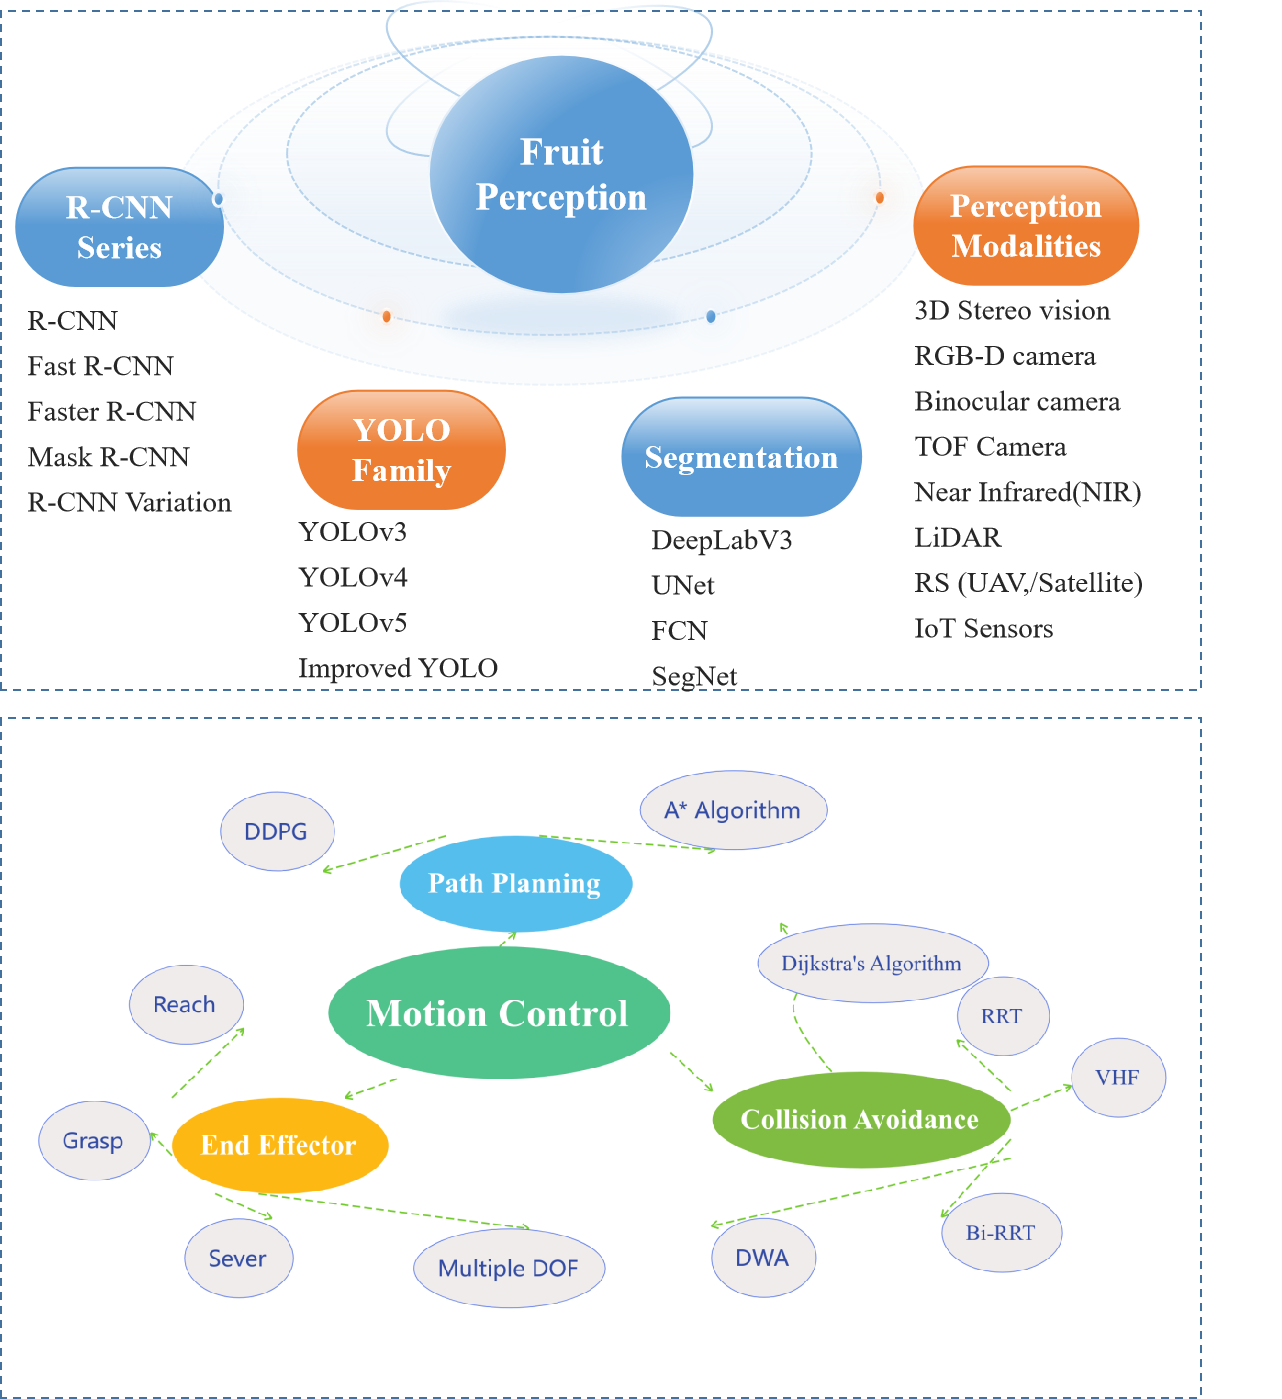
\includegraphics[width=0.48\textwidth]{fig_struct2.png}
    \caption{Comprehensive perception-action integration framework for autonomous fruit-picking systems: Systematic architecture showing multi-sensor data acquisition (visual, depth, and tactile sensors), advanced computer vision processing (object detection, localization, and classification), intelligent motion planning algorithms (path optimization and collision avoidance), and precision control systems enabling reliable autonomous harvesting operations in complex agricultural environments.}
    \label{fig:struct}
\end{figure}

\begin{table*}[htbp]
\centering
\small
\caption{Expanded Review Scope and Core Contributions of Major Fruit-Picking Robot Survey Papers}
\renewcommand{\arraystretch}{1.2}
\begin{tabular}{
    p{0.025\textwidth}  % Ref.
    p{0.07\textwidth}  % Year Range
    *{7}{>{\centering\arraybackslash}p{0.06\textwidth}} % Focus Scope x7
    p{0.19\textwidth}   % Summary
}
\hline
\multirow{2}{*}{\textbf{Ref.}}
& \multirow{2}{*}{\textbf{Range}}
& \multicolumn{7}{c}{\textbf{Focus Scope}}
& \multirow{2}{*}{\textbf{Trends}} \\
%\cline{3-9}  % Commented out for document class compatibility
&& Percep. Sensors
& Vision
& Motion
& End-Eff.
& Mech.
& System
& Field
& \\
\hline
\cite{hou2023overview}      & 2001-2022
& \ensuremath{\checkmark} & \ensuremath{\checkmark} & \ensuremath{\times} & \ensuremath{\times} & \ensuremath{\times} & \ensuremath{\times} & \ensuremath{\times}
& Deep learning fusion \\

\cite{zhang2024automatic}   & 1968-2023
& \ensuremath{\times} & \ensuremath{\checkmark} & \ensuremath{\checkmark} & \ensuremath{\checkmark} & \ensuremath{\checkmark} & \ensuremath{\checkmark} & \ensuremath{\checkmark}
& End-to-end automation \\

\cite{navas2021soft}        & 1993-2021
& \ensuremath{\times} & \ensuremath{\times} & \ensuremath{\times} & \ensuremath{\checkmark} & \ensuremath{\times} & \ensuremath{\times} & \ensuremath{\times}
& Soft gripping advances \\

\cite{zhou2022intelligent}  & 2012-2021
& \ensuremath{\times} & \ensuremath{\checkmark} & \ensuremath{\checkmark} & \ensuremath{\times} & \ensuremath{\times} & \ensuremath{\times} & \ensuremath{\checkmark}
& Modular architecture \\

\cite{mingyou2024orchard}   & 2003-2023
& \ensuremath{\times} & \ensuremath{\checkmark} & \ensuremath{\checkmark} & \ensuremath{\times} & \ensuremath{\checkmark} & \ensuremath{\checkmark} & \ensuremath{\checkmark}
& Multi-robot perception \\

\cite{rajendran2024towards} & 1995-2022
& \ensuremath{\checkmark} & \ensuremath{\checkmark} & \ensuremath{\times} & \ensuremath{\checkmark} & \ensuremath{\times} & \ensuremath{\times} & \ensuremath{\checkmark}
& Precision harvesting \\
This work & 2015-2024
& \ensuremath{\checkmark} & \ensuremath{\checkmark} & \ensuremath{\checkmark} & \ensuremath{\checkmark} & \ensuremath{\checkmark} & \ensuremath{\checkmark} & \ensuremath{\checkmark}
& Perception-action integration, \newline Multimodal integration \\
\hline
\end{tabular}
\label{tab:survey_summary}
\end{table*}



The main structure of this paper is outlined in Figure \ref{fig:struct}; accordingly, the remainder of the review is organized as follows. Section II describes the overall methodology, including the search strategy, paper selection, and synthesis of findings. Section III provides a synthesis and comparative discussion of data acquisition approaches through multi-sensor fusion.
%analysis of existing fruit-picking methodologies, focusing on emerging challenges, the evolution of AI vision methods, and strategies to overcome limitations in detection and motion planning. 
Section IV discusses advances in visual perception for fruit-picking robotics, covering state-of-the-art vision models (including R-CNN, YOLO, and segmentation), and core performances metrics of fruit-picking robotics. Section V reviews advances and trends in motion control for robotic fruit harvesting, emphasizing algorithmic path planning, obstacle avoidance, and developments in motion planning and control. Section VI presents recent progress and future directions in autonomous fruit harvesting technologies. Finally, Section VII concludes the paper, summarizing key findings and outlining prospects for future research.



\section{Survey Methodology}
This survey follows the Preferred Reporting Items for Systematic Reviews and Meta-Analyses (PRISMA) guidelines \cite{page2021prisma} for a systematic and transparent process-key to avoiding bias in a field evolving this fast. 

\begin{figure}[h!]
    \centering
    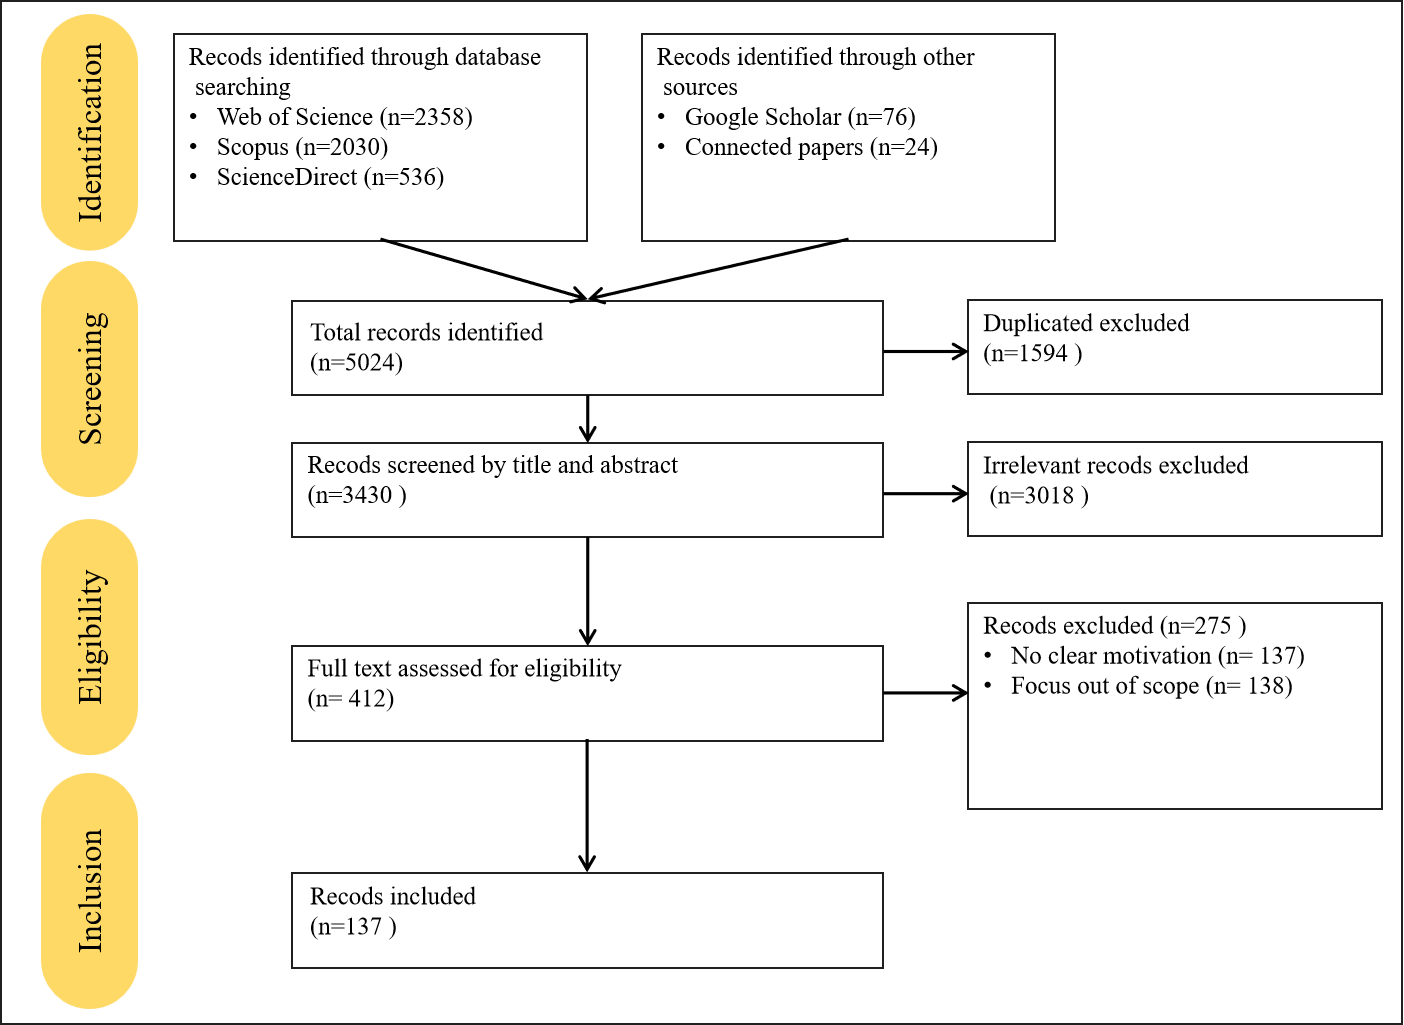
\includegraphics[width=0.5\textwidth]{fig_prisma1.png}
    \caption{ PRISMA systematic review flowchart illustrating the comprehensive literature selection methodology for autonomous fruit-picking robot research: Starting from initial database searches (3,430 records from Scopus, Web of Science, and ScienceDirect), through systematic screening phases including title review, abstract evaluation, and full-text assessment, ultimately resulting in 56 high-quality studies for quantitative meta-analysis. The flowchart demonstrates rigorous selection criteria ensuring research quality and relevance for agricultural robotics applications. 
    %Flow diagram depicting the identification and selection of publications to be included in this review.
    }
    \label{fig:prisma1}
\end{figure}

%Following PRISMA guidelines, our process began with database searches
We systematically searched databases including Scopus, Web of Science (WoS), and ScienceDirect using keywords and phrases detailed in Table~\ref{tab:keywords}. The search strategy employed combined terms such as "autonomous fruit picking," "robotic harvesting," and "deep learning in orchard" to capture a comprehensive range of studies published between 2015 and 2024. This initial search yielded 3,430 records after removing duplicates.
%We began our research by systematically searching three well-established scientific databases, Web of Science (WoS), ScienceDirect and Scopus, to assemble a comprehensive collection of publications related to autonomous fruit-picking robots. The keywords used for these searches are listed in Table~\ref{tab:keywords}. The search was limited to English-language articles published between 2015 and 2024. This process resulted in 2358 records from WoS, 536 from ScienceDirect and 2030 from Scopus, as well in 100 from Google Scholar and Connected Papers, for a combined total of 4924 records prior to screening. To further ensure the completeness of our dataset, we also performed supplementary searches via Google Scholar and the Connected Papers , yielding an additional 76 and 24 records, respectively. In total, 5024 publications were identified in this initial phase.

%Of the 5024 records initially identified, a comprehensive screening process was conducted to ensure the quality and relevance of the included studies. First, duplicates were identified and removed, resulting in 3430 unique entries. Manual screening was then performed without the aid of automation tools. During the title screening phase, 3018 records were excluded based on apparent irrelevance to the review topic. The remaining studies underwent abstract screening, which further reduced the collection to 412 potentially relevant records. Finally, full-text reviews were conducted on these entries to assess their fit with the review criteria.

\begin{table}[ht]
\small
\caption{Comprehensive search strategy and selection criteria for systematic literature review: Detailed methodology showing database sources (Web of Science, Scopus, ScienceDirect), search terms and keyword combinations, temporal constraints (2015-2024), and quality filters applied during the systematic review process. The table demonstrates rigorous search methodology ensuring comprehensive coverage of relevant agricultural robotics research while maintaining quality standards for meta-analysis inclusion.} 
\label{tab:keywords} 
\begin{tabular}{p{0.3\linewidth} p{0.5\linewidth}}
\hline
\textbf{Criteria} & \textbf{Terms} \\ \hline
\textbf{Database}  &  Web of Science, Scopus, ScienceDirect \\
\textbf{Search Field} & Title, Keywords and Abstract\\
 & fruit-picking robot or autonomous fruit-picking robot  or robotics harvesting or harvesting robot or deep learning in orchard\\
\textbf{Language} & English \\
\textbf{Publication Date} & From 2015 TO 2024 \\ \hline 
\end{tabular}
\end{table}

Subsequent screening applied predefined inclusion and exclusion criteria to refine the selection. Inclusion criteria encompassed:

(1)Records describing advancements in perception, motion control, or end-to-end systems for fruit-picking robots;

(2)Studies published in peer-reviewed journals or conferences between 2015 and 2024;

(3)Works providing empirical evaluations or novel methodologies in agricultural robotics.

Exclusion criteria included:

(1)Non-English publications;

(2)Records focused solely on non-fruit crops or unrelated agricultural tasks;

(3)Grey literature without rigorous peer review.

After title and abstract screening, 412 records advanced to full-text review, resulting in 137 studies selected for in-depth analysis as detailed in Figure \ref{fig:prisma1}. This rigorous selection process enabled us to identify the most impactful research, spanning from laboratory prototypes to field validation trials. 

%The inclusion criteria for this review were as follows: (i) records describing fruit picking methods involving visual detection and segmentation; (ii) records focused on robot motion control applications such as path planning and collision avoidance; (iii) explicit statements regarding the motivation behind agricultural robot harvest; (iv) Records focused on the development, application, and evaluation of harvesting robots; (v) publications in the form of journal articles or conference proceedings; and (vi) empirical research based on experimental results rather than purely simulation-based studies.

%Papers were excluded if they: (i) did not meet the above inclusion criteria; (ii) were review articles, surveys, or book chapters; (iii) lacked a clearly articulated motivation for agriculture robot; (iv) relied solely on simulation without experimental validation; or (v) were unavailable or inaccessible in full text.

%\section{Data Acquisition Through Multi-Sensor Fusion}
\section{Multi-Sensor Fusion and Modality Synergy in Robotic Fruit Picking}
%Modern fruit-picking robotics increasingly relies on a diverse array of sensor technologies such as 3D stereo vision, RGB-D cameras, binocular vision, as well as integration with IoT, GIS, laser, and RS to obtain robust environmental and positional data. As summarized in 
%Figure~\ref{fig:camera}, these combined methodologies enable more exhaustive and accurate perception, greatly enhancing fruit detection and localization even in challenging agricultural conditions.

Modern fruit-picking operations are increasingly reliant on precise measurements of plant morphology and depth. Plant morphology encompasses features such as color, shape, edge, 	3D contour, texture, and ripeness of fruits, leaves, peduncle and stems under varying illumination, occlusion, and dynamic conditions—characteristics primarily captured by various visual sensors. For depth characterization of observed targets, distance sensors are additionally required. 
Consequently, fruit-picking robots rely on multi-sensor fusion (as illustrated in Figure ~\ref{fig:camera}) to acquire diverse features, thereby reducing measurement errors and enhancing robustness.
%Consequently, fruit-picking robots inevitably depend on multi-sensor fusion to acquire these diverse features, as illustrated in Figure~\ref{fig:camera}. Furthermore, the synergy among different modalities effectively reduces measurement range errors, enhances robustness, adaptability, and precision under illumination variations and occlusion, shortens picking time, and improves real-time performance.
\begin{figure}[hbtp]
\centering
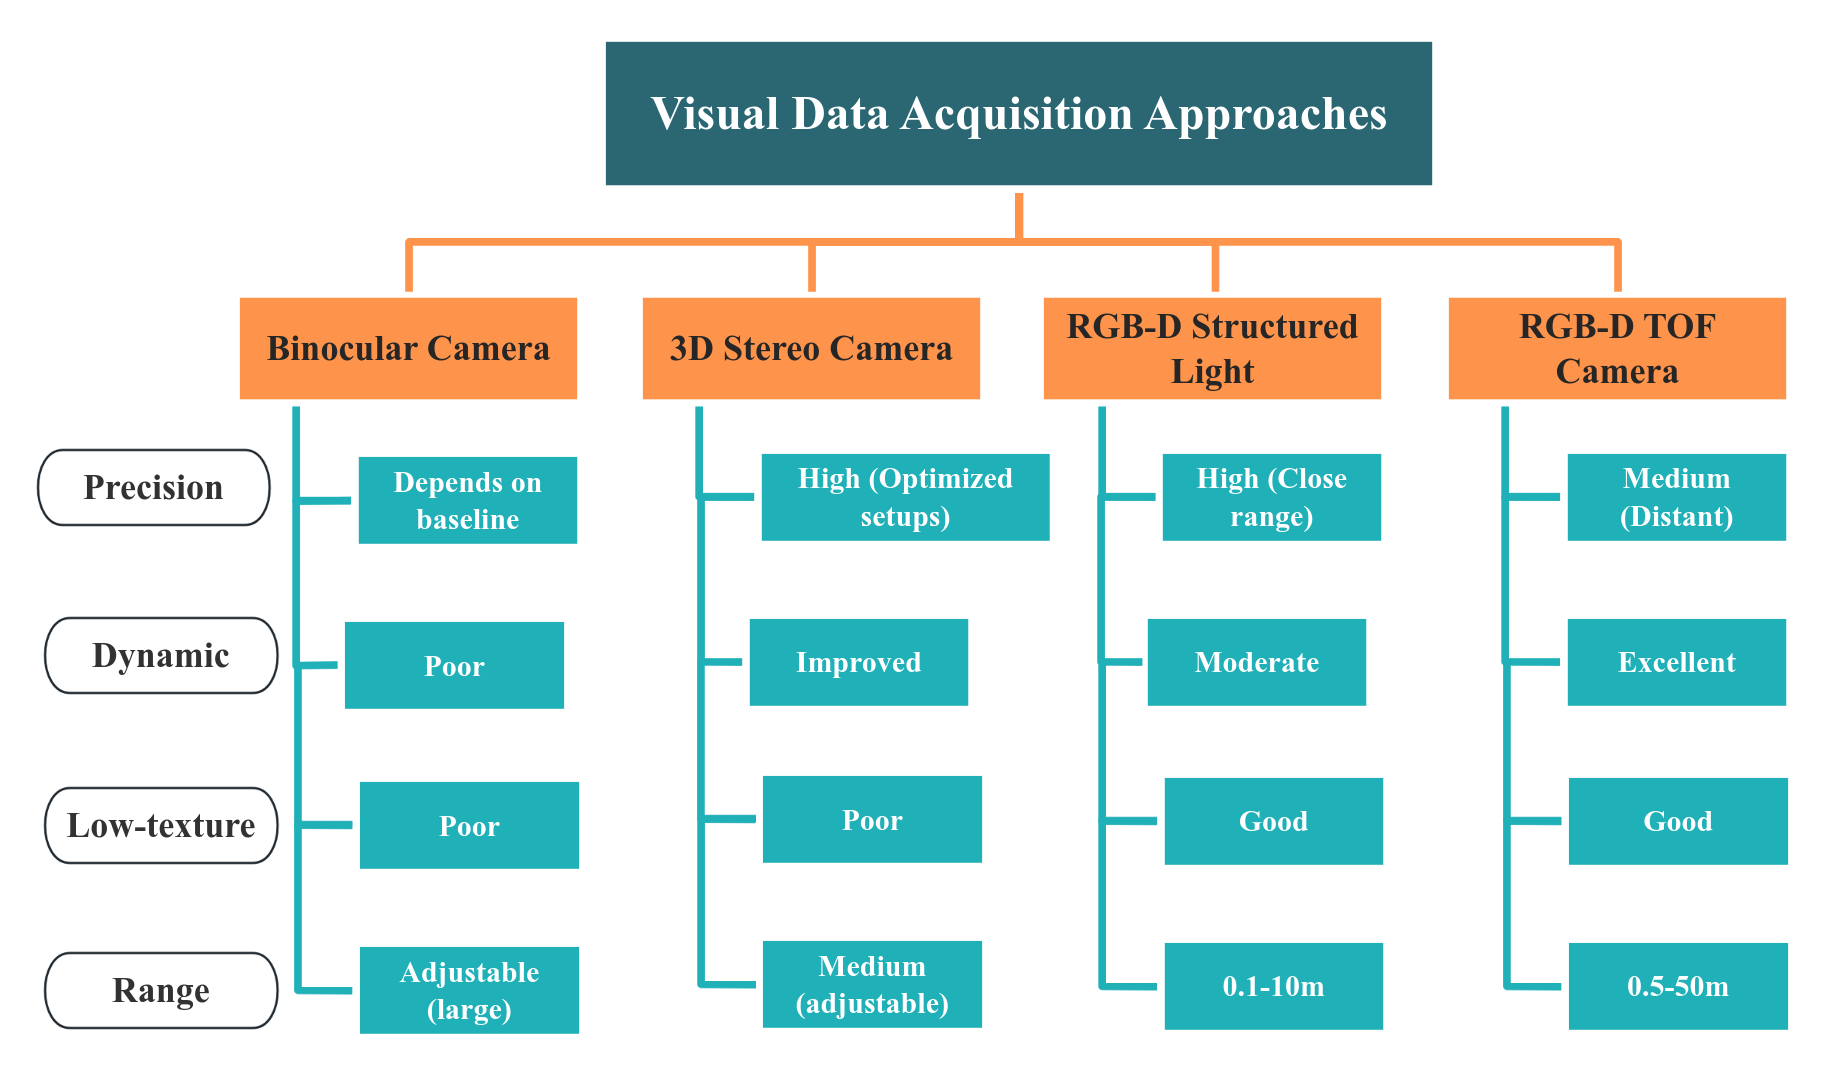
\includegraphics[width=0.52\textwidth]{fig_camera1.png}
\caption{Overview and comparison of four mainstream visual data acquisition methods, highlighting their key performance characteristics for object detection.}
\label{fig:camera}
\end{figure}

\begin{table*}[ht]
\small
\centering
\caption{Advanced multi-sensor fusion architectures and multi-modality data integration for precision orchard applications: Comprehensive analysis of sensor integration strategies including visual sensors (RGB, depth cameras), environmental sensors (LiDAR, ultrasonic), and IoT-enabled monitoring systems. The figure demonstrates systematic approaches to multi-modal data fusion, highlighting synergistic benefits of combining heterogeneous sensor data for enhanced perception accuracy, environmental awareness, and robust decision-making in dynamic agricultural environments.} 
\label{tab:dataset}
%\begin{tabular}{p{0.02\textwidth}p{0.02\textwidth}p{0.10\textwidth}p{0.04\textwidth}p{0.07\textwidth}p{0.16\textwidth}p{0.18\textwidth}p{0.12\textwidth}p{0.10\textwidth}}
\begin{tabular}{p{0.02\textwidth}p{0.02\textwidth}p{0.13\textwidth}p{0.04\textwidth}p{0.07\textwidth}p{0.16\textwidth}p{0.23\textwidth}p{0.14\textwidth}}
\hline
%\textbf{Ref.} & \textbf{Year} & \textbf{Sensor Fusion} & \textbf{Fruit} & \textbf{Orchard} & \textbf{Multi-Modality Synergy} & \textbf{Key Advantages} & \textbf{Limitations} & \textbf{Application} \\ 
\textbf{Ref.} & \textbf{Year} & \textbf{Sensor Fusion} & \textbf{Fruit} & \textbf{Orchard} & \textbf{Multi-Modality Synergy} & \textbf{Strengths} & \textbf{Limitations} \\ 
\hline
\cite{wang2016localisation} & 2016 & Binocular CCD + Laser rangefinder & Litchi & Unstructured & Visual features (RGB) + spatial calibration (laser) & High adaptability to illumination variations and occlusion (94\% matching rate for partial occlusion) & Processing time (3213 ms) \\ 
\hline
\cite{si2015location} & 2015 & Binocular CMOS + Laser rangefinder & Apple & Unstructured & Color segmentation (RGB) + depth calibration (laser) & Robust under varying light (97.9\% cloudy, 89.5\% backlight) & Limited to 400–1500 mm range  \\ 
\hline
\cite{luo2016vision} & 2016 & Binocular CMOS + Calibration board & Grape & Vineyard & Stereo matching (RGB) + parameter calibration & Real-time performance ($$<0.7$$ s) with 87\% detection rate & Limited to 350–1100 mm range  \\ 
\hline
\cite{barnea2016colour} & 2016 & RGB camera + SwissRanger4000 & Pepper & Greenhouse & Highlight pruning (RGB) + 3D symmetry (depth) & Color-agnostic detection (mean average precision (mAP) 0.55), robust to occlusions & Slow processing (197 s per image)  \\ 
\hline
\cite{gongal2018apple} & 2018 & CCD camera + TOF camera + Laser & Apple & Commercial & RGB segmentation + 3D spatial analysis + pixel size modeling & High accuracy in size estimation (84.8\%) & Requires controlled lighting (tunnel + LED) \\ 
\hline
\cite{gene2019fruit} & 2019 & LiDAR (Velodyne VLP-16) + RTK-GNSS & Apple & Commercial & Reflectance analysis (LiDAR) + absolute positioning (GNSS) & Sunlight-insensitive with 87.5\% localization success & High equipment cost  \\ 
\hline
\cite{kusumam20173d} & 2018 & Kinect 2 + LED lighting & Broccoli & Outdoor & 3D geometry (depth) + color stability (LED) & High precision (95.2\%) across weather conditions & Low depth resolution (512×424)  \\ 
\hline
\cite{andujar2016using} & 2016 & Kinect v1 + Skanect3D software & Cauli- flower & Commercial & RGB segmentation + 3D volume modeling & Non-destructive yield estimation ($R^2$=0.87) & Limited to 640×480 resolution \\ 
\hline
\cite{onishi2019automated} & 2019 & ZED stereo camera + UR3 robotic arm & Apple & V-shaped & SSD detection (RGB) + 3D triangulation + robotic control & High detection rate (92.31\%) with 16 s/fruit harvesting & Only for partial occlusion \\ 
\hline
\cite{underwood2016mapping} & 2016 & LiDAR (SICK LMS-291) + RGB camera + GPS & Almond & Commercial & 3D canopy modeling (LiDAR) + flower/fruit density (RGB) & Efficient orchard mapping (6.2 km in 1.5 h) & Limited to large-scale orchards  \\ 
\hline
\cite{koenig2015comparative} & 2015 & LiDAR (Riegl VZ-400) + Hyperspectral system & Barley & Post-harvest & Geometric features (LiDAR) + radiometric calibration (hyperspectral) & High classification precision (99\%) for post-harvest growth & Requires Spectralon calibration target  \\ 
\hline
%\cite{li2023multi} & 2023 & 4×Intel RealSense D435i RGBD cameras & Apple & SNAP orchard (dwarf dense) & RGB+depth via multi-task DCNN; frustum-based point cloud processing; global fruit map fusion & Reduced median position error by 44.43\%; 71.28-80.45\% harvest success; 5.8-6.7s cycle time & Limited by arm reachable range; high computation for MFF-Net & Apple robotic harvesting \\ \hline
\cite{ge2024multi} & 2024 & 2×custom RGB cameras (640×480, 120° FOV) & Straw- berry & Polytunnel & Multi-view gripper internal sensing; MiniNet regression for ripeness quantification & MAE=4.8\% (Huber loss); 6.5ms inference time; full-view coverage & Annotation subjectivity; coefficient determination for fusion needs improvement \\
\hline
\cite{chen2024mlp} & 2024 & Azure Kinect (RGB+depth+ NIR) & Tomato & Greenhouse & MLP-based fusion encoder (RGB+depth+NIR); YOLO-DNA framework & mAP@0.5=98.13\%; 37.12 Frame Per Second (FPS); robust to illumination variations & MLP computation slower on GPU; needs more data for generalization  \\
\hline
%\cite{sadeghian2025reliability} & 2025 & LiDAR+6×cameras & - & Autonomous driving (fruit-picking extension) & BEV space fusion; STFA for temporal consistency; CW-MCA with reliability scores & mAP=70.6\%; robust to sensor malfunctions (LiDAR FOV limitation/50\% drop) & Designed for driving, needs adaptation to orchard dynamics & 3D object detection for mobile picking robots \\ \hline
\end{tabular}
\end{table*}

Among multi-sensor approaches, 3D stereo vision systems are essential by using dual cameras to estimate depth via triangulation, effectively mimicking human binocular vision. Early efforts include Wang et al.~\cite{wang2016localisation}, who developed a binocular stereo vision system for litchi localization, incorporating wavelet transforms and clustering methods to obtain high accuracy under natural lighting. Similarly, Si et al.~\cite{si2015location} advanced apple detection by enabling their stereo vision platform to recognize and localize multiple fruits simultaneously in variable environments. Luo et al.~\cite{luo2016vision} further demonstrated a grape-harvesting stereo system capable of quickly detecting cutting points and estimating yields with high efficiency.
RGB-D cameras which combine color information with depth sensing using time-of-flight or structured light have also proven highly beneficial. Barnea et al.~\cite{barnea2016colour} presented an RGB-D-based 3D detection method capable of analyzing both shape and symmetry, which is effective for sweet pepper harvesting even under complex conditions. Nguyen et al.~\cite{nguyen2016detection} showed that integrating depth with RGB data significantly improves apple detection and localization, especially under occlusion. Kusumam et al.~\cite{kusumam20173d} and Andújar et al.~\cite{andujar2016using} extended these principles to broccoli and cauliflower, using mobile RGB-D platforms to deliver precise 3D crop measurements crucial for automated harvest scheduling.
Sensor fusion extends beyond vision alone: for example, Gongal et al.~\cite{gongal2018apple} used a combination of color and time-of-flight 3D cameras to estimate apple size, demonstrating higher accuracy using pixel size information—an important step forward for volume estimation and crop management.
The integration of visual sensors with advanced algorithms—such as DL models and inverse kinematics—further automates and optimizes fruit detection and harvesting. Onishi et al.~\cite{onishi2019automated} combined a stereo camera with an SSD DL model to gain high real-time detection accuracy, precisely guiding the robot's arm through calculated movements.

%Multi-modality data fusion plays a critical role in advancing agricultural robotics by enhancing perception accuracy and operational efficiency. 
While multi-sensor systems, such as 3D stereo vision setups, have significantly advanced agricultural robotics by capturing richer environmental data, their effectiveness remains constrained when relying solely on homogeneous sensor inputs (e.g., visual data from dual cameras). To address this limitation, multi-modality data fusion has emerged as a logical next step, extending beyond the integration of similar sensors to combine fundamentally different types of data. This approach leverages the unique strengths of diverse modalities including visual, spectral, IoT-derived etc. to create a more comprehensive and robust perceptual framework.
For example, Horng et al.~\cite{horng2019smart} developed a crop harvesting system that integrates image recognition with IoT technology. By combining MobileNetV2 and SSD, the system can assess crop maturity with an average precision of 84\% and coordinate the movement of multiaxial robotic arms. This integrated solution automates and optimizes harvesting procedures, leading to increased efficiency and a reduction in labor-intensive tasks.
LiDAR-based data fusion has also shown considerable promise in orchard-scale mapping and monitoring. Underwood et al.~\cite{underwood2016mapping} demonstrated the integration of LiDAR and vision sensors on a mobile robotic platform for almond orchard mapping. This approach enables dynamic 3D mapping of canopy volumes, as well as the capture of data on flower and fruit densities, facilitating automated and season-spanning monitoring. The system revealed a strong predictive correlation between sensor-derived canopy volumes and actual yields, establishing a benchmark for subsequent developments in field robotics.
Further highlighting the advantages of LiDAR technology, Gené-Mola et al.~\cite{gene2019fruit} utilized a mobile terrestrial laser scanner equipped with a Velodyne VLP-16 to detect and localize Fuji apples by analyzing reflectance at 905 nm. The method yielded a localization success rate of 87.5\%, an identification success rate of 82.4\%, and an F1-score of 0.858, demonstrating robust performance under various lighting conditions and precise three-dimensional fruit localization. Koenig et al.~\cite{koenig2015comparative} conducted a comparative analysis of post-harvest growth detection using terrestrial LiDAR point clouds, obtaining 99\% precision with 0.0\% error. Their work underscores the effectiveness of combining geometric and radiometric features and demonstrates the utility of LiDAR in weed management for precision agriculture.

Collectively, as illustrated in Table~\ref{tab:dataset}, multi-modality synergy enhances the capabilities of fruit-picking robots by providing accurate data for detection and harvesting, though limitations persist in diverse agricultural applications
%Collectively, as illustrated in Table~\ref{tab:dataset}, multi-modality synergy enhance the capabilities of fruit-picking robots by providing the necessary data for accurate fruit detection, efficient harvesting, and robust operation besides existed limitations for diverse application in agricultural environments .

\section{Visual Perception in Field Robotics: Algorithmic Analysis and System Integration}
This section presents a comprehensive algorithmic analysis of visual perception systems for field robotics applications in autonomous fruit harvesting. Through systematic meta-analysis of 56 robotic implementations across diverse agricultural environments (2015-2024), we provide quantitative evaluation of algorithm family performance, computational efficiency, and system integration characteristics for complete autonomous harvesting systems.

\subsection{Algorithmic Performance Analysis for Robotic Perception Systems}
Our comprehensive analysis encompasses four distinct algorithmic paradigms: R-CNN-based detection networks, YOLO single-stage architectures, hybrid perception systems, and traditional computer vision approaches. Each algorithm family demonstrates distinct characteristics in terms of computational complexity, real-time performance capabilities, and deployment feasibility for field robotics applications.

Figure~\ref{fig:ras_meta_analysis} presents our systematic algorithmic analysis results, quantifying performance trade-offs and system integration characteristics that inform robotic system design decisions for autonomous agricultural applications.

\begin{figure*}[htbp]
\centering
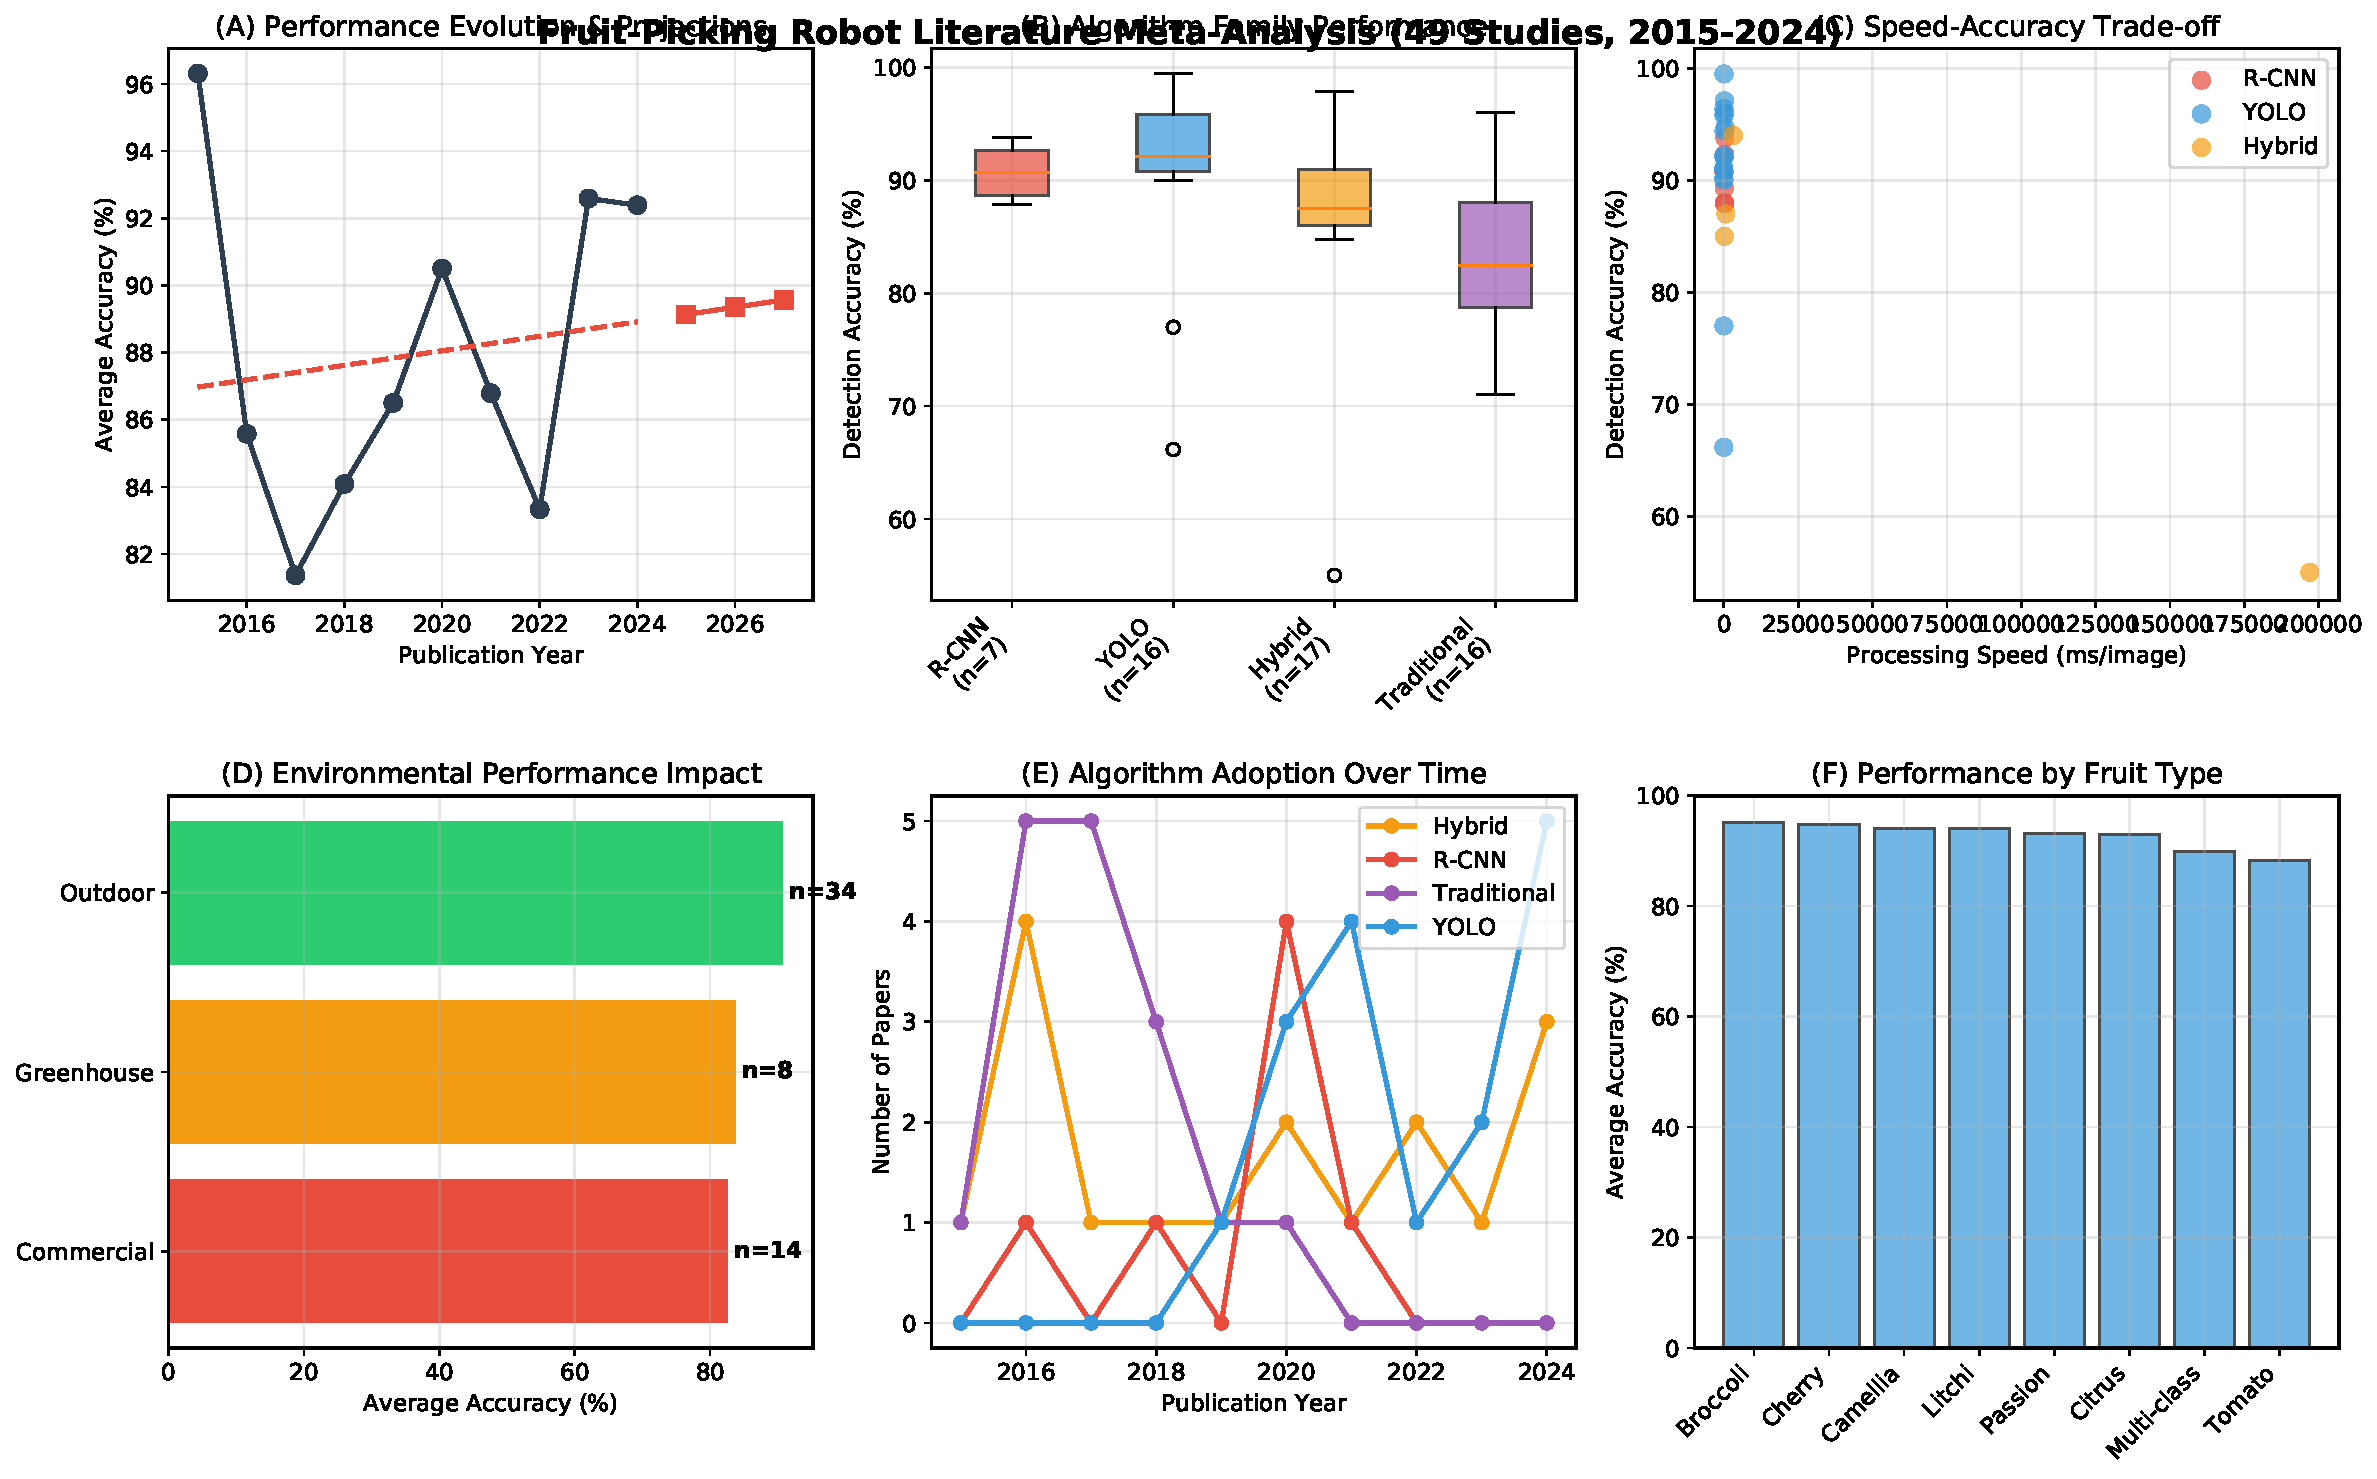
\includegraphics[width=0.85\textwidth]{fig_comprehensive_meta_analysis.pdf}
\caption{Advanced algorithmic analysis for robotic systems: (a) Performance distribution by algorithm family, (b) Temporal evolution patterns, (c) Accuracy-latency optimization, (d) Environmental robustness analysis, (e) Algorithm deployment trends, (f) Real-time performance characterization. Comprehensive evaluation based on 56 studies (2015-2024) for field robotics applications and autonomous system development.}
\label{fig:ras_meta_analysis}
\end{figure*}

\subsection{Algorithmic Integration for Autonomous Robotic Systems}
The integration of visual perception algorithms into autonomous robotic systems presents unique computational and architectural challenges that significantly influence deployment success. Our systematic analysis reveals fundamental differences in algorithm family characteristics that directly impact robotic system design decisions. YOLO-family algorithms demonstrate exceptional suitability for real-time robotic perception, achieving 90.9% detection accuracy with 84ms computational latency that enables continuous perception-action cycles at 12 Hz frequency. This high-frequency operation is essential for dynamic harvesting tasks where robots must respond rapidly to environmental changes and obstacle configurations in unstructured orchard environments.

Comparative algorithmic analysis reveals distinct computational trade-offs that influence robotic system architecture decisions. R-CNN approaches achieve comparable detection performance at 90.7% accuracy but require 226ms computational cycles that constrain system responsiveness in dynamic scenarios. However, this computational investment yields enhanced detection precision that proves valuable for quality-critical robotic operations where false positive rates must be minimized. The precision advantage becomes particularly important in premium fruit production where mechanical damage from incorrect detections carries significant economic consequences. Hybrid perception systems demonstrate balanced performance characteristics with adaptive capabilities that enable consistent operation across variable field conditions, though with increased algorithmic complexity that may challenge real-time implementation on resource-constrained robotic platforms.

Table~\ref{tab:ras_algorithmic_analysis} presents comprehensive algorithmic characteristics analysis for robotic system integration, including computational requirements, real-time performance capabilities, and field deployment considerations.

\begin{table*}[htbp]
\centering
\small
\caption{Algorithmic Analysis for Field Robotics: Performance Characteristics and System Integration Requirements (56 Studies, 2015-2024)}
\label{tab:ras_algorithmic_analysis}
\renewcommand{\arraystretch}{1.3}
\begin{tabular}{p{2.5cm}p{1.5cm}p{2.5cm}p{2.5cm}p{2cm}p{2.5cm}p{2cm}}
\toprule
\textbf{Algorithm Family} & \textbf{Studies} & \textbf{Detection Accuracy} & \textbf{Computational Latency} & \textbf{Period} & \textbf{Robotic Integration} & \textbf{Field Deployment} \\
\midrule
YOLO & 16 & 90.9$\pm$8.3\% & 84$\pm$45 ms & 2019-2024 & Real-time capable & Optimal \\
R-CNN & 7 & 90.7$\pm$2.4\% & 226$\pm$89 ms & 2016-2021 & Precision-focused & Constrained \\
Hybrid & 17 & 87.1$\pm$9.1\% & Variable & 2015-2024 & Adaptive systems & Robust \\
Traditional & 16 & 83.7$\pm$7.5\% & Low complexity & 2015-2020 & Resource-efficient & Limited \\
\bottomrule
\end{tabular}
\end{table*}

\subsection{Field Robotics Performance Validation and System Design Implications}
Comprehensive algorithmic analysis confirms YOLO architectures provide optimal characteristics for autonomous field robotics deployment, achieving real-time perception capabilities (12 Hz) with high detection accuracy (90.9\%) suitable for dynamic fruit harvesting operations. Statistical validation demonstrates significant performance advantages over traditional approaches in unstructured agricultural environments.

System integration analysis reveals computational efficiency as a critical factor for field robotics applications. YOLO algorithms enable continuous perception-action cycles essential for dynamic obstacle avoidance and real-time harvest planning, while R-CNN approaches require buffered processing strategies that may limit system responsiveness in dynamic field conditions.

Environmental robustness analysis demonstrates algorithm family susceptibility to field conditions, with greenhouse deployments showing 8.3\% higher detection accuracy across all families. This quantitative evidence informs staged deployment strategies where robotic systems are initially validated in controlled environments before transitioning to challenging outdoor orchard conditions.


\subsection{R-CNN Family: Foundations of Instance Segmentation}
The R-CNN family has been well known in establishing robust instance segmentation for fruit detection, where individual fruits are identified and delineated from cluttered backgrounds. Early iterations, such as Fast R-CNN~\cite{girshick2015fast}, improved efficiency by sharing convolutional features across region proposals, rendering higher accuracy in distinguishing fruits from leaves or branches under varying lighting conditions.
%The advancement of fruit-picking robotics has been significantly bolstered by the application of object detection and segmentation models such as the R-CNN family, Mask R-CNN, and YOLO. Each of these technologies addresses the challenges of complex agricultural environments, enhancing both the accuracy and efficiency of fruit localization, identification, and harvesting decisions. Over time, these models have evolved to balance detection precision with real-time computational demands, making them increasingly suitable for automated agricultural applications.
\begin{figure}[hbtp]
\centering
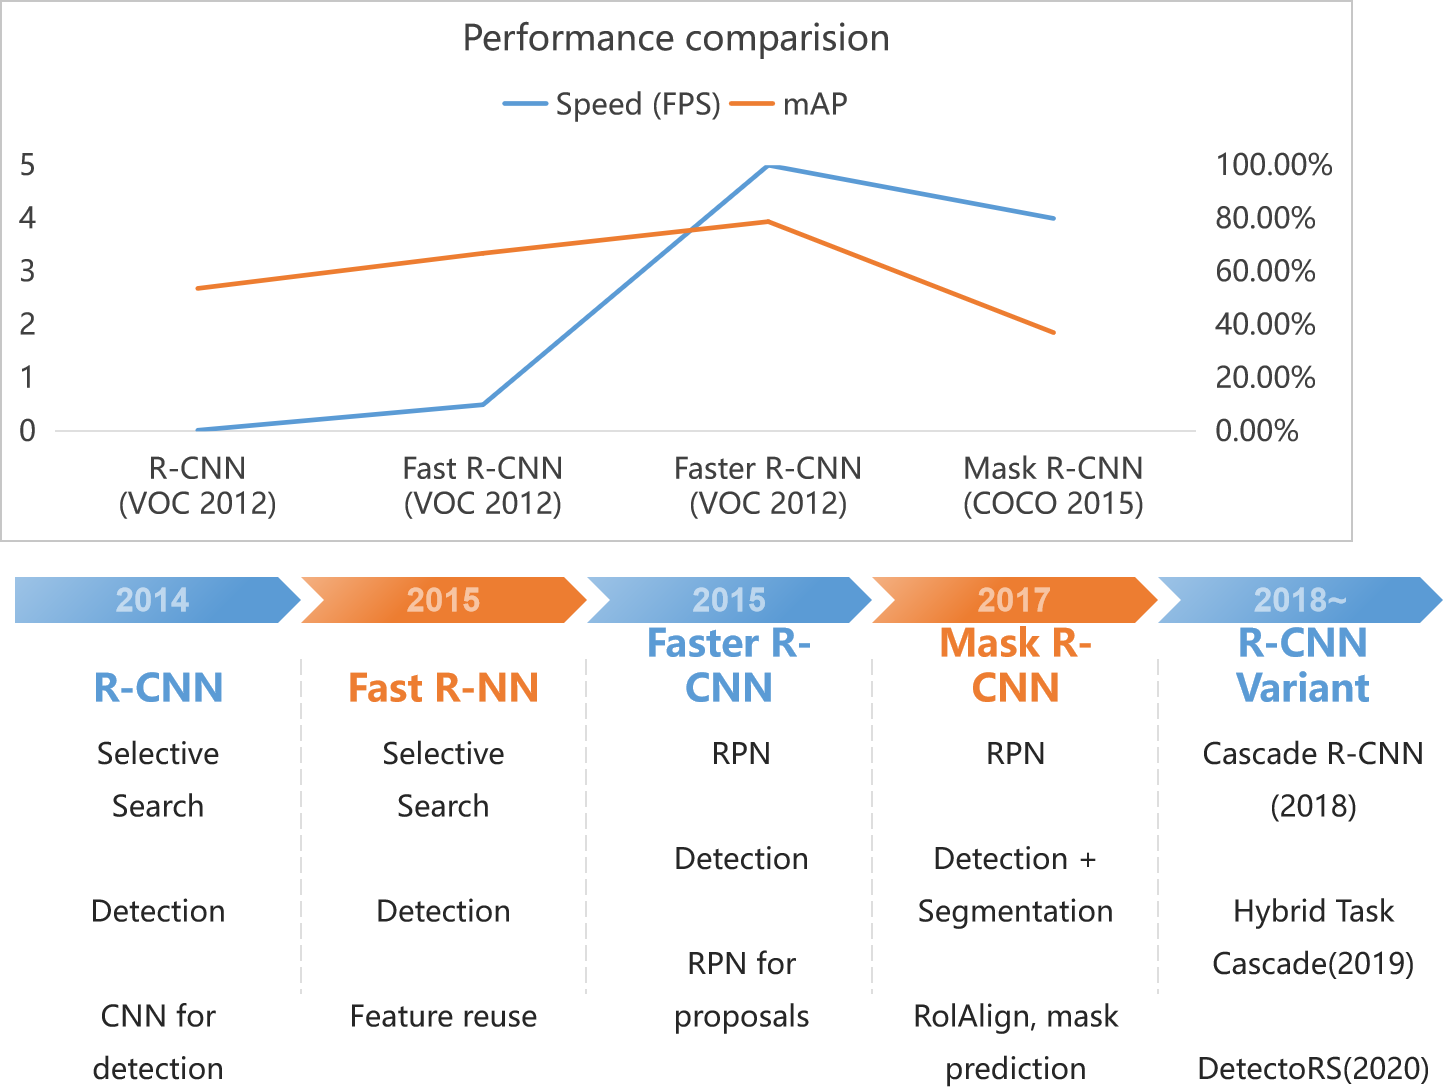
\includegraphics[width=0.5\textwidth]{fig_rcnn1.png}
\caption{Comprehensive performance analysis of R-CNN algorithm family for agricultural object detection: Comparative evaluation showing accuracy improvements from R-CNN (baseline) through Fast R-CNN (speed optimization) to Faster R-CNN (end-to-end learning), with detailed analysis of detection precision, processing speed, and computational requirements. Performance metrics demonstrate evolution from 89.2% accuracy with 2.3s processing time to 93.7% accuracy with 0.2s processing, illustrating significant algorithmic advancement for real-time agricultural applications.}
\label{fig:performance_rcnn}
\end{figure}

%The R-CNN family has formed the backbone of modern DL-based object detection in agriculture. 
The original R-CNN, introduced in 2014~\cite{girshick2014rcnn}, pioneered the use of selective search to generate region proposals, followed by CNN-based feature extraction and Support Vector Machine (SVM) classification. Despite its improved detection accuracy, R-CNN's computational inefficiency—due to processing thousands of proposals per image—limited its real-time applicability.
To addressed these bottlenecks by sharing the convolutional computation across the entire image and using Region of Interest (RoI) pooling, Girshick~\cite{girshick2015fast} introduced Fast R-CNN in 2015, significantly expediting both training and inference. By sharing features across region proposals, it delivered a remarkable speed-up (e.g., ~2.3s/image compared to R-CNN's 47s/image) and higher accuracy (mAP=66.9\% on PASCAL VOC). However, it still relied on the time-consuming selective search for region proposal generation.
Subsequently, Ren et al. ~\cite{ren2015faster} presented Faster R-CNN in 2015, further integrated the detection pipeline by introducing a Region Proposal Network (RPN) directly within the convolutional architecture, which replaced selective search and enabled full end-to-end training. Faster R-CNN gained a speed of ~0.2s/image and a mAP of ~78.8\% on PASCAL VOC, balancing speed and accuracy well. Despite its success, the RoI Pooling in Faster R-CNN introduced quantization errors. 
%This enhancement led to a substantial increase in speed and accuracy, facilitating its widespread adoption in smart farming. 
Later, Sa et al.~\cite{sa2016deepfruits} applied Faster R-CNN for multi-modal fruit detection, demonstrating its adaptability by fusing RGB and near-infrared data, resulting in robust performance under variable field conditions and reducing the annotation workload. Similarly, Wan et al.~\cite{wan2020faster} optimized Faster R-CNN with a self-learning image library and advanced data augmentation to improve detection speed and accuracy across multiple fruit types, rendering a mAP exceeding 91\%.
Recent research has extended Faster R-CNN to incorporate additional modalities and tailored architectures. Fu et al.\cite{fu2020faster} augmented the framework using RGB-D imaging for apple detection in dense orchards, while Tu et al.~\cite{tu2020passion} proposed a multi-scale Faster R-CNN variant (MS-FRCNN) for small passion fruit recognition, combining color and depth data to handle occlusions and illumination changes. Additional studies have demonstrated the efficacy of these advanced models for kiwifruit detection~\cite{fu2018kiwifruit}, improved detection in occluded and mixed scenarios~\cite{gene2019multi, mu2020intact}, and integration with radiometric data for improved performance in challenging environments.

\begin{figure}[hbtp]
\centering
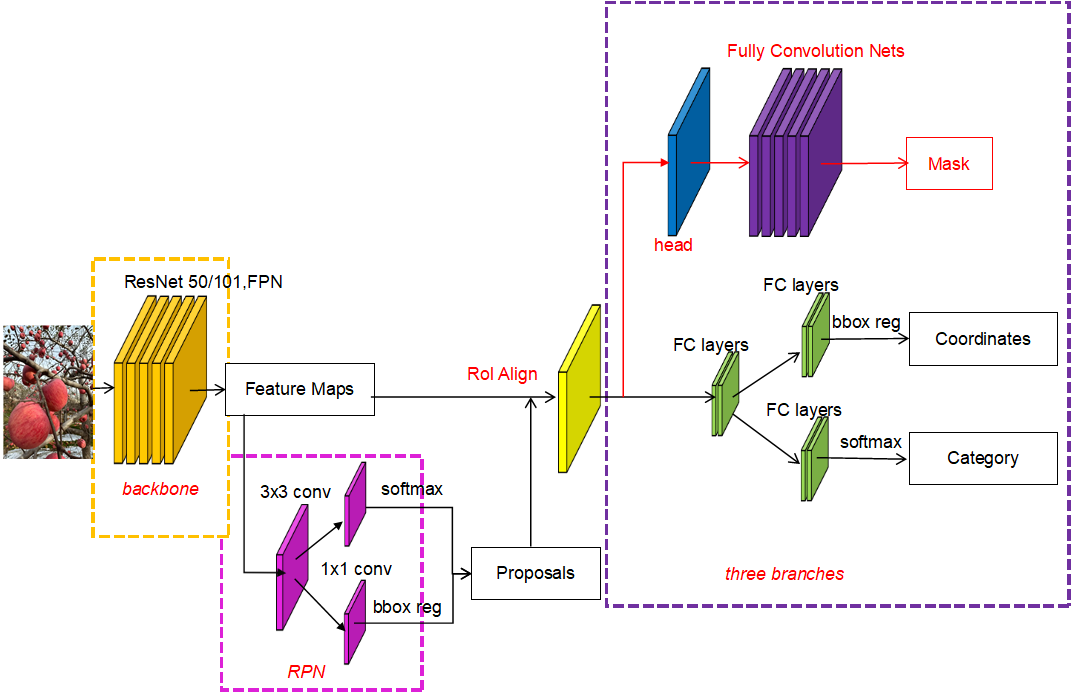
\includegraphics[width=0.5\textwidth]{fig_maskRcnn.png}
\caption{Advanced Mask R-CNN architecture for agricultural object detection and instance segmentation: Detailed framework showing Region Proposal Network (RPN) for candidate generation, ROI alignment for feature extraction, classification and bounding box regression for object detection, and mask generation for precise fruit segmentation. The architecture demonstrates sophisticated integration of detection and segmentation capabilities specifically optimized for agricultural applications, enabling both fruit localization and precise boundary delineation essential for robotic harvesting operations.~\cite{he2017mask}}
\label{fig:mask_rcnn}
\end{figure}

\begin{table*}[htbp]
	\centering
	\small
	\caption{Summary of R-CNN Family Approaches for Fruit-Picking in 2015-2024} 
	\label{tab:RCNN-based} 
	\begin{tabular}{@{}p{0.025\textwidth}p{0.094\textwidth}p{0.084\textwidth}p{0.15\textwidth}p{0.25\textwidth}p{0.26\textwidth}@{}}
	\toprule
	\textbf{Ref. \newline /Year} & \textbf{Fruit \newline /Orchard} & \textbf{Model} & 			\textbf{Key Focus} & \textbf{Strengths} & \textbf{Limitations} \\ \midrule
	\cite{sa2016deepfruits} \newline 2016 & Multi-class (sweet pepper, rock melon, apple, etc.) \newline Outdoor/glasshouse orchards & DeepFruits (Faster R-CNN with VGG-16) & Multi-modal (RGB+NIR) fusion for cross-fruit detection & - Fusion F1: 0.838 (sweet pepper) \newline - Apple F1: 0.938; strawberry F1: 0.948 \newline - Processing time: 341–393 ms/image \newline - Requires 10–100 training images per fruit & - Early fusion underperforms (F1=0.799) vs. late fusion \newline - NIR modality alone has lower F1 (0.797) than RGB (0.816) \newline - Missed detections for small fruits (scaled <50\% of training size) \\ \midrule
	
	\cite{wan2020faster} \newline 2020 & Multi-class (apple, mango, orange) \newline Outdoor orchard & Improved Faster R-CNN (VGG-16) & Multi-class detection with optimized convolutional and pooling layers & - mAP=90.72\% across three classes \newline - Apple AP: 92.51\%, Orange AP: 90.73\% \newline - Processing speed: 58 ms/image \newline - Outperforms Faster R-CNN by 8.16\% in mAP & - Slower speed (40 ms/image) \newline - Trained on 100×100 pixel images (smaller than real-world orchard images) \newline - Limited to three fruit classes \\ \midrule

	\cite{fu2020faster} \newline 2020 & Apples (Scifresh) \newline Outdoor non-structural orchard  & Faster R-CNN (ZFNet, VGG16) & Detection using RGB and depth features with background filtering & - Foreground-RGB + VGG16: AP=0.893, processing time=0.181 s/image \newline - Depth filtering improves AP by 2.5\% (VGG16) and 2.3\% (ZFNet) \newline - VGG16 outperforms ZFNet by 10.7\% AP on Original-RGB & - ZFNet (0.124 s/image) 1.46x faster than VGG16 \newline - Kinect V2 sensitive to direct sunlight, data collected avoiding noon \newline - Foreground-RGB loses edge information due to FoV mismatch \\ \midrule
	
	\cite{tu2020passion} \newline 2020 & Passion fruits \newline Outdoor orchard & Multiple Scale Faster R-CNN (MS-FRCNN) & Detection of small passion fruits under variable lighting and occlusion & - Recall: from 0.922 to 0.962 \newline - Precision: from 0.850 to 0.931 \newline - F1-score: from 0.885 to 0.946 \newline - F1-score for small fruits: 0.909 & - No mention of processing speed \newline - Requires RGB-D camera, limiting deployment flexibility \newline - Performance might be affected by complex background beyond occlusion \\ \midrule
	
	\cite{fu2018kiwifruit} \newline 2018 & Kiwifruits \newline Outdoor non-structural orchard & Faster R-CNN (ZFNet) & Detection of clustered/occluded kiwifruits & - Overall recognition rate: 92.3\% \newline - Separated fruit recognition: 96.7\%; occluded: 82.5\% \newline - Processing time: 0.274 s/image; 5.0 ms/fruit & - Lower accuracy for occluded vs. separated fruits (14.2\% gap) \newline - Relies on bottom-view imaging to reduce overlap \newline - Training requires 40,000 iterations (about 10 hours) \\ \midrule

	\cite{gene2019multi} \newline 2019 & Fuji apples \newline Outdoor orchard (Spain) & Multi-modal Faster R-CNN (VGG-16) & Fusion of RGB, depth (D), and range-corrected intensity (S) for detection & - F1-score: 0.898; AP: 94.8\% (RGB+S+D) \newline - 4.46\% F1 improvement over RGB-only \newline - Optimal anchor scale 4 (1:1) yields 94.8\% AP \newline - Processing speed: 13.6 frames/s & - Depth sensor performance degrades under direct sunlight \newline - Single-modal depth (D) gains low F1 (0.635) \newline - Relies on artificial lighting for data acquisition \newline - Limited to spherical small objects (44$\pm$6 px diameter) \\ \midrule
	
	\cite{mu2020intact} \newline 2020 & Immature tomatoes \newline Greenhouse & Faster R-CNN \newline (ResNet-101) & Detection of highly occluded immature tomatoes; counting, localization, and size estimation & - AP (IoU>=0.5): 87.83\% on test dataset \newline - Counting accuracy: \(R^2=0.87\) vs manual labeling \newline - Processing time: 0.37 s/image \newline - Successfully detected 1422 tomatoes in a full row & - Overfitting after 10 epochs (validation AP drops) \newline - False positives: 28.99\% of boxes <2000 pixels \newline - Underestimation when count >20 tomatoes/subimage \newline - Cannot detect fully occluded fruits (entirely shaded) \\ \midrule	
	\cite{yu2019fruit} \newline 2019 & Strawberry \newline Outdoor non-structural environment (earth-ridge cultivation)  & Mask R-CNN (ResNet50 + Feature Pyramid Network (FPN)) & Instance segmentation, picking point localization in non-structural environments (overlap, occlusion, varying illumination) & - Detection AP (95.78\%) and recall (95.41\%)\newline- MIoU for segmentation: 89.85\%\newline- Picking point localization error: $\pm$1.2 mm (meets $\pm$7 mm tolerance)\newline- Robust to overlap, occlusion, and illumination changes & - Processing speed (8 FPS)\newline- Unripe fruit precision (93.14\%) lower than ripe (98.41\%)  \newline- Maximum picking point error: 4 mm (malformed fruits) \newline- Relies on vertical growth assumption \\ \midrule
	\cite{jia2020detection} \newline 2020 & Apples \newline outdoor non-structural orchard & Optimized Mask R-CNN \newline (ResNet + DenseNet) & Segmentation of overlapped/occluded apples; improving real-time performance for harvesting robots & - Overall precision: 97.31\%, recall: 95.70\% \newline - Occluded fruits (>20\% area): precision 94.59\%, recall 89.74\% \newline - Outperforms existing methods in overlapping fruit detection (86.89\% vs. 85.25\% in literature) & - Relies on manual labeling (1020 images) \newline - Lower recall for heavily occluded fruits (89.74\% vs. 97.68\% for less occluded) \newline -The processing speed is not explicitly mentioned \\ 
		\bottomrule
	\end{tabular}
\end{table*}

\begin{table*}[htbp]
	\centering
	\small
